\subsection{Getting verbose!}

Although we use colours in SDMs to indicate when an element is to be matched (black), created (green), or destroyed (red), sometimes makes it sense to indicate
these binding operators via explicit stereotypes (i.e., in preparation for black-and-white printouts of a model).

\begin{enumerate}
  
\item[$\blacktriangleright$] Open the relevant diagram in the EA editor window and then depending on what type it is, press the \texttt{Verbose} button in
either the \texttt{eMoflon SDM Functions} or \texttt{eMoflon TGG Function} (Fig.~\ref{ea:changeVStatus}).

\vspace{0.5cm}

\begin{figure}[htbp]
\begin{center}
  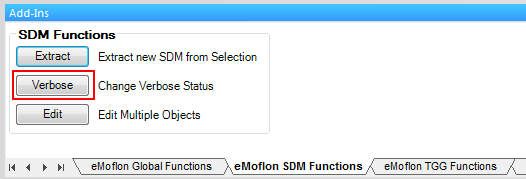
\includegraphics[width=0.8\textwidth]{ea_changeVerboseStatus}
  \caption{Verbal change of links}  
  \label{ea:changeVStatus}
\end{center}
\end{figure}

\item[$\blacktriangleright$] This will add small \texttt{++} or \texttt{-} symbols next to the line or element in question (Fig.~\ref{ea:verboseSymbols}). Press
the button again to deactivate these indicators.

\begin{figure}[htbp]
\begin{center}
  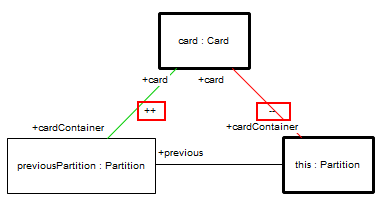
\includegraphics[width=0.7\textwidth]{ea_verboseSymbols}
  \caption{Verbal change of links}  
  \label{ea:verboseSymbols}
\end{center}
\end{figure}

\end{enumerate}
